%!TEX root = ../systemnahe-programmierung.tex

\chapter{Einleitung}\label{einleitung}

\begin{figure}[htbp]
\centering
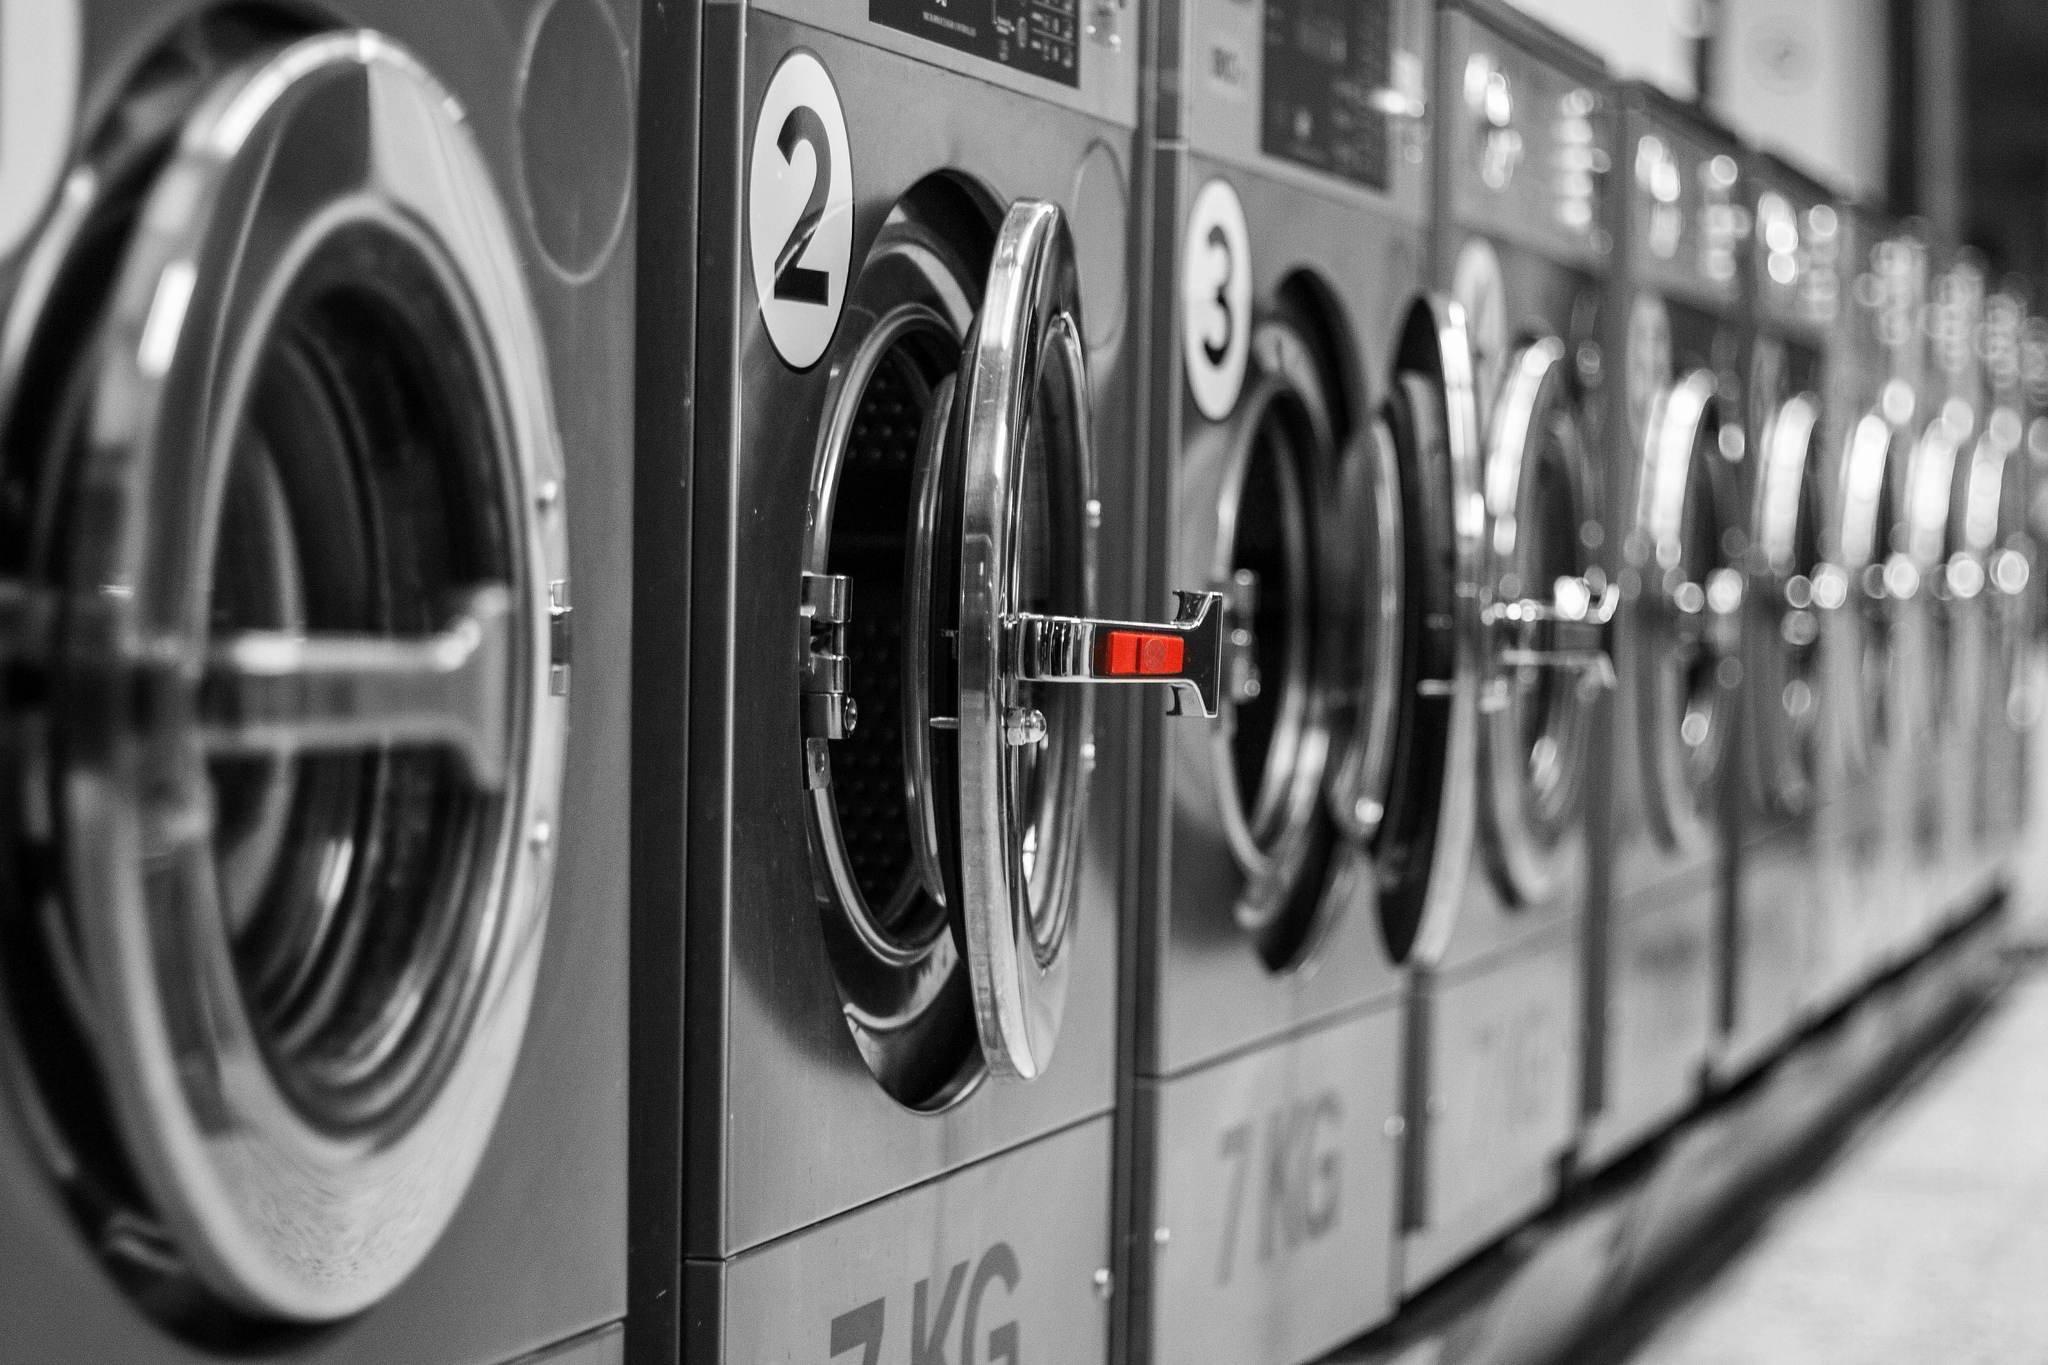
\includegraphics{images/washing-maschine}
\caption[Microcontroller im Alltag]{Microcontroller im Alltag\footnotemark{}}
\end{figure}
\footnotetext{Choose only one, https://www.flickr.com/photos/97922031@N05/15884820461,
  Einsichtsnahme: 31.01.2015}

Systemnahe Programmierung beschäftigt sich mit der Erstellung beziehungsweise Programmierung von
Software, die Teil des Betriebssystemes oder sehr eng mit diesem verbunden ist.

Die Software dient hierbei als Abstraktionsschicht zwischen Hardware und Betriebssystem, welche
leichten Zugriff auf einfache Funktionen des Systems bietet.

Heutzutage nimmt Systemnahe Programmierung einen sehr hohen Stellenwert ein. Sie ist mittlerweile in
unserem Alltag in Form von Microcontrollern mit verschiedensten Einsatzgebieten vertreten.
Microcontroller sind in Autos, Mobiltelefonen, Waschmaschinen, elektrischen Zahnbürsten,
Fernbedienungen und vielen anderen Geräten zu finden.

Die Systeme sind nicht nur omnipräsent sondern der Markt wächst immer mehr. Durch den Aufstieg von
Wearables und dem Drang alle Geräte miteinander zu verbinden, werden immer mehr Microcontroller
verbaut. So kam auch der Anstieg von 12\% in 2014 zu Stande, der für 2015 mit 15\% noch höher
ausfallen soll\footnote{(o.V.) (2015) Microcontroller market 2015,
  http://www.emittsolutions.com/section/market-analysis/market\_analysis\_microcontroller.html,
  Einsichtnahme: 27.01.2015.}.